\documentclass[12pt,a4paper,twoside,openright,titlepage,final]{article}
\usepackage{fontspec}
\usepackage{amsmath}
\usepackage{amsfonts}
\usepackage{amssymb}
\usepackage{makeidx}
\usepackage{graphicx}
\usepackage[hidelinks,unicode=true]{hyperref}
\usepackage[spanish,es-nodecimaldot,es-lcroman,es-tabla,es-noshorthands]{babel}
\usepackage[left=3cm,right=2cm, bottom=4cm]{geometry}
\usepackage{natbib} 
\usepackage{microtype}
\usepackage{ifdraft}
\usepackage{verbatim}
\usepackage[spanish]{cleveref}
\usepackage[obeyDraft]{todonotes}
\ifdraft{
	\usepackage{draftwatermark}
	\SetWatermarkText{BORRADOR}
	\SetWatermarkScale{0.7}
	\SetWatermarkColor{red}
}{}
\usepackage{booktabs}
\usepackage{longtable}
\usepackage{calc}
\usepackage{array}
\usepackage{caption}
\usepackage{subfigure}
\usepackage{footnote}
\usepackage{url}
\usepackage{tikz}

\usetikzlibrary{positioning}

\tikzset{%
  zeroarrow/.style = {-stealth,dashed},
  onearrow/.style = {-stealth,solid},
  c/.style = {circle,draw,solid,minimum width=2em,
        minimum height=2em},
  r/.style = {rectangle,draw,solid,minimum width=2em,
        minimum height=2em}
}


\setsansfont[Ligatures=TeX]{texgyreadventor}
\setmainfont[Ligatures=TeX]{texgyrepagella}

%*******************************************************
%                 NO MODIFICAR
\newcommand*{\FSfont}[1]{%
  \fontencoding{T1}\fontfamily{#1}\selectfont}

\newlength{\tpheight}\setlength{\tpheight}{0.9\textheight}
\newlength{\txtheight}\setlength{\txtheight}{0.9\tpheight}
\newlength{\tpwidth}\setlength{\tpwidth}{0.9\textwidth}
\newlength{\txtwidth}\setlength{\txtwidth}{0.9\tpwidth}
\newlength{\drop}
%*******************************************************

% Crea una portada con los siguientes parámetros
%
% #1 : Título 
% #2 : Subtítulo
% #3 : Subsubtítulo
% #4 : Autor(es)
% #5 : Lugar
%

\newcommand*{\portada}[5]{
\begin{titlepage}
\begingroup
\vspace*{1cm}
\drop = 0.2\txtheight
\centering
\vfill
{\Huge \scshape #1}\\[\baselineskip]
{\Large \textbf{#2}}\\[\baselineskip]
{\Large \scshape #3}\\[\baselineskip]
\vspace*{0.3cm}
{\large \textit{#4}}\\[0.5\drop]

\includegraphics[scale=0.35]{./imagenes/logoURJC.jpg}
\vspace*{1.5cm}

{\large \scshape #5, \today} \par
\begin{center}
\end{center}
\vfill\null
\endgroup
\end{titlepage}
}
 %*****************************************************
 


\author{José Ignacio Escribano}

\title{Práctica final}

\setlength{\parindent}{0pt}

\begin{document}

\pagenumbering{alph}
\setcounter{page}{1}

\portada{Práctica final}{Ingeniería de la Decisión}{Ruta óptima para llegar al trabajo}{José Ignacio Escribano}{Móstoles}

\listoffigures
\thispagestyle{empty}
\newpage

\listoftables
\thispagestyle{empty}
\newpage

\tableofcontents
\thispagestyle{empty}
\newpage


\pagenumbering{arabic}
\setcounter{page}{1}

\section{Introducción}

Habitualmente, nos desplazamos para llegar al trabajo, y tenemos, en general, varias formas de ellas hasta él. Los medios de transporte que tendremos disponibles en el problema serán coche, metro, autobús y Cercanías Renfe. Nuestro objetivo es llegar lo más rápido posible, es decir, minimizar el tiempo de llegada hasta el trabajo. Supondremos que nuestro trabajo se encuentra en la ciudad de Madrid, y hasta él tenemos una distancia de 30 kilómetros, independientemente del medio de transporte elegido. Preferimos los medios terrestres (coche y autobús) sobre los medios subterráneos (metro y Cercanías). Además de llegar lo antes posible, también queremos tener la máxima comodidad, que sea lo más barato y que contamine lo menos posible. Si se elige los servicios de transporte (metro, autobús o Cercanías) se quiere minimizar el número de transbordos.\\

\section{Resolución del problema}

En las siguientes secciones resolveremos el problema siguiendo el ciclo del análisis de decisión (Figura~\ref{fig:ciclo}).

\begin{figure}[tbph!]
	\centering
	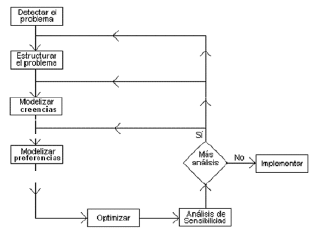
\includegraphics[width=0.5\linewidth]{imagenes/ciclo}
	\caption{Ciclo del análisis de decisión}
	\label{fig:ciclo}
\end{figure}

\subsection{Estructuración del problema}

Para resolver el problema comenzamos identificando los distintos elementos que componen el problema, esto es, identificamos los factores de incertidumbre, los objetivos conflictivos, la influencia del tiempo, los decisores y los grupos afectados:\\

\begin{itemize}
	
	\item \textbf{Factores de incertidumbre}
	
	\begin{itemize}
		\item Condiciones meteorológicas (lluvia, nieve, hielo, sol, ...), precio del combustible, precio de los servicios de transporte, nivel de contaminación, la predicción meteorológica
	\end{itemize}
	
	\item \textbf{Objetivos conflictivos}
	
	\begin{itemize}
		\item Minimizar el tiempo de llegada, minimizar el coste, maximizar la comodidad, preferencia de medios terrestres sobre medios subterráneos, minimizar el número de transbordos, minimizar las emisiones de CO2.
	\end{itemize}
	
	\item \textbf{Influencia del tiempo}
	
	\begin{itemize}
		\item Condiciones meteorológicas, precio del combustible, precio de los servicios de transporte (tanto a corto como a largo plazo), día y hora en la que nos encontremos (por ejemplo, no es lo mismo ir a trabajar un domingo que habrá menos tráfico por la carretera, que un lunes por la mañana que seguramente habrá retenciones), apertura de nuevas carreteras o nuevos servicios en los medios de transporte.
	\end{itemize}
	
	\item \textbf{Decisores}
	
	\begin{itemize}
		\item Nosotros mismos
	\end{itemize}
	
	\item \textbf{Grupos afectados}
	
	\begin{itemize}
		\item Nosotros mismos, usuarios de los servicios de transporte, usuarios de coches, ciudadanos de Madrid (por la contaminación)
	\end{itemize}
\end{itemize}

Una vez que tenemos identificamos los elementos del problema, procedemos a crear el diagrama de influencia.\\

En primer lugar, ponemos las incertidumbres, los objetivos y las decisiones (elegir medio de transporte) en GeNIe (Figura~\ref{fig:diagrama_1}).\\
 

\begin{figure}[tbph!]
\centering
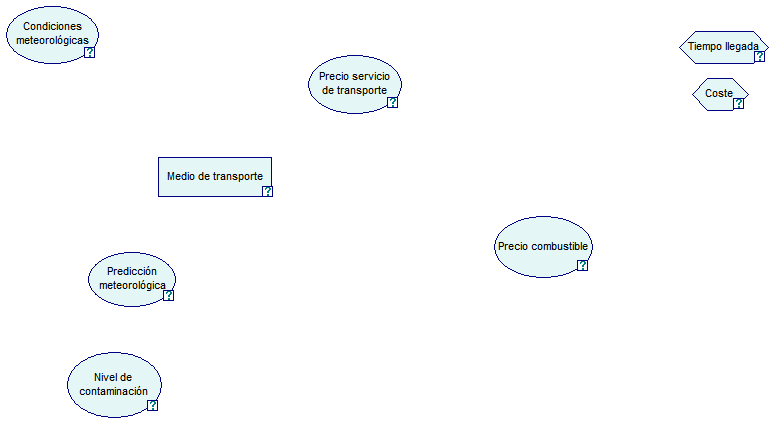
\includegraphics[width=0.9\linewidth]{imagenes/diagrama_1}
\caption{Primer boceto del diagrama de influencia}
\label{fig:diagrama_1}
\end{figure}

En este primer boceto, sólo introducimos los objetivos de minimizar el coste y el tiempo de llegada. Más adelante consideraremos los demás objetivos.\\

Nos queda introducir los arcos entre los nodos. Para ello, consideramos las influencias entre cada uno de los nodos (Figura~\ref{fig:diagrama_2}).\\

Comencemos con el nodo de Condiciones meteorológicas: hay un arco entre este nodo y nivel de contaminación ya que las condiciones meteorológicas condicionan el nivel de contaminación. También hay un arco hacia el nodo de valor Tiempo llegada ya que la meteorología influye en el tiempo que tardaremos en llegar al trabajo.\\

En el nodo Predicción meteorológica, tenemos un arco hacia Condiciones meteorológicas, ya que la condiciones meteorológica vendrán determinadas por la predicción meteorológica.\\

El precio del combustible condiciona al Precio del servicio de transporte, y ambos precios afectan al objetivo del coste.\\

Para tomar la decisión, conocemos la predicción meteorológica, las condiciones meteorológicas actuales, los precios del combustible y de los servicios de transporte, y el nivel de contaminación.

\begin{figure}[tbph!]
	\centering
	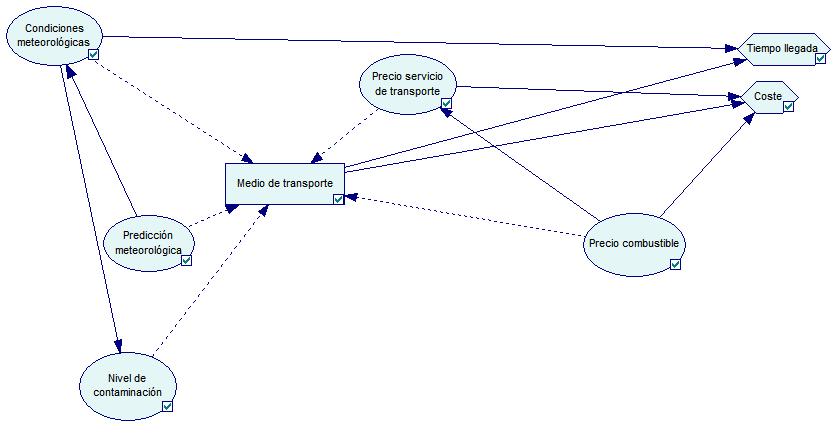
\includegraphics[width=0.9\linewidth]{imagenes/diagrama_2}
	\caption{Diagrama de influencia con los arcos}
	\label{fig:diagrama_2}
\end{figure}

\subsection{Modelización de creencias}

Ahora procedemos a asignar probabilidades a los nodos de azar.\\

En primer lugar consideraremos los estados de los nodos Condiciones y Predicción meteorológica. Éstos serán cuatro: lluvia, nieve, niebla y despejado.\\

Se sabe que la predicción de lluvia se dio el 15\% de los casos, nieve en el 5\%, niebla en el 10\% y despejado el 70\% (Tabla~\ref{tbl:prob_pred_met}).\\   

\begin{table}[htbp!]
\centering
\caption{Estados y probabilidades del nodo Predicción meteorológicas}
\label{tbl:prob_pred_met}
\begin{tabular}{@{}cc@{}}
\toprule
Predicción & Probabilidad \\ \midrule
Lluvia     & 0.15         \\
Nieve      & 0.05         \\
Niebla     & 0.10         \\
Despejado  & 0.70         \\ \bottomrule
\end{tabular}
\end{table}

También se conocen las probabilidades de que se produzcan las condiciones meteorológicas actuales dadas las predicción (Tabla~\ref{tbl:condicionadas}).

\begin{table}[htbp!]
	\centering
	\caption{Probabilidades de las condiciones condicionadas a las predicciones meteorológicas}
	\label{tbl:condicionadas}
	\begin{tabular}{@{}ccccc@{}}
		\toprule
		Condiciones\textbackslash Predicción & Lluvia & Nieve & Niebla & Despejado \\ \midrule
		Lluvia                               & 0.80   & 0.30  & 0.30   & 0.10      \\
		Nieve                                & 0.01   & 0.60  & 0.20   & 0.01      \\
		Niebla                               & 0.10   & 0.05  & 0.40   & 0.01      \\
		Despejado                            & 0.09   & 0.05  & 0.10   & 0.88      \\ \bottomrule
	\end{tabular}
\end{table} 

En el nodo Precio combustible consideramos dos estados: precio alto y bajo. Diremos que el precio es alto si nos cuesta 1 litro de gasolina más de 1.20 euros. En caso contrario, tenemos un precio bajo.\\

Se conoce que el 70\% de los días de los últimos cinco años, el precio del combustible ha estado alto. El 30\% restante ha tenido un precio bajo.\\

Con el precio del transporte tenemos, de nuevo, dos estados: precio alto y bajo. Consideraremos que el precio del transporte es alto si la media aritmética del coste los transportes públicos (metro, autobús y Cercanías) es mayor a 3 euros. En caso contrario, el precio es bajo.\\

Se saben las probabilidades del precio del transporte público, dado el precio del combustible (Tabla~\ref{tbl:condicionadas_2}).

\begin{table}[htbp!]
	\centering
	\caption{Probabilidades del precio del transporte condicionadas al precio del combustible}
	\label{tbl:condicionadas_2}
	\begin{tabular}{@{}ccc@{}}
		\toprule
		Precio transporte \textbackslash Precio combustible & Precio alto & Precio bajo \\ \midrule
		Precio alto                                         & 0.75        & 0.50        \\
		Precio bajo                                         & 0.25        & 0.50        \\ \bottomrule
	\end{tabular}
\end{table}

El último nodo que nos queda es el Nivel de contaminación. Tenemos dos estados contaminación alta y baja. Consideramos que el nivel es alto si se tiene una medida superior a 700 ppm (partes por millón).\\

Por último, conocemos la probabilidad del nivel de contaminación dadas las condiciones meteorológicas (Tabla~\ref{tbl:condicionadas_3}).\\

\begin{table}[htbp!]
	\centering
	\caption{Probabilidades del nivel de contaminación dadas las condiciones meteorológicas}
	\label{tbl:condicionadas_3}
	\begin{tabular}{@{}ccccc@{}}
		\toprule
		Nivel contaminación \textbackslash Condiciones meteorológicas & Lluvia & Nieve & Niebla & Despejado \\ \midrule
		Nivel alto                                                    & 0.70   & 0.50   & 0.40   & 0.30       \\
		Nivel bajo                                                    & 0.25   & 0.50   & 0.60   & 0.70      \\ \bottomrule
	\end{tabular}
\end{table}

Todos las probabilidades anteriores las introducimos en el modelo de GeNIe.

\subsection{Modelización de preferencias}

Ahora modelizamos nuestras preferencias con el software Web-HIPRE.\\

En primer lugar, definimos nuestro modelo jerárquico de objetivos. Nuestro objetivo principal será llegar al trabajo, que a su vez, tiene tres subobjetivos: el económico, el confort y los sociales. En el primero se encuentra el coste y el tiempo de llegada; en el segundo, los transbordos, el tiempo de espera, las personas del habitáculo y el tipo de transporte (que a su vez puede ser terrestre o subterráneo); y los últimos, formado por los ruidos y la contaminación. La Figura~\ref{fig:modelo_jerarquico_objetivos} muestra la jerarquía completa (junto con las alternativas) una vez introducidas en Web-HIPRE.

\begin{figure}[tbph!]
	\centering
	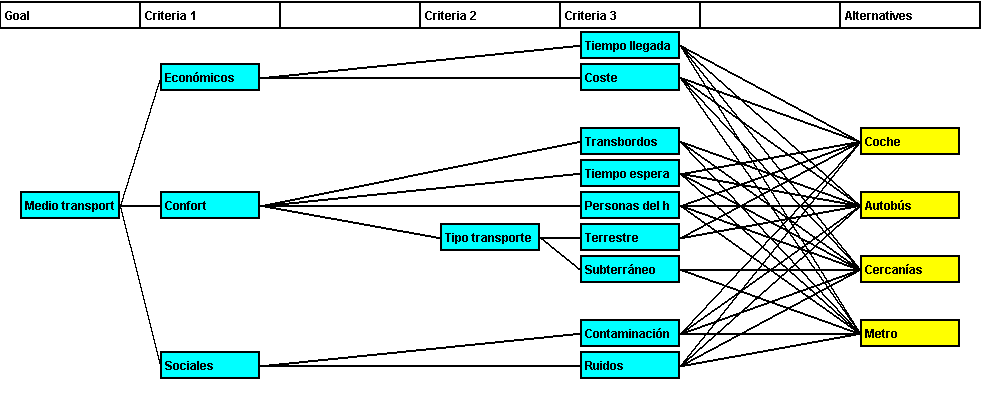
\includegraphics[width=0.9\linewidth]{imagenes/modelo_jerarquico_objetivos}
	\caption{Modelo jerárquico de objetivos}
	\label{fig:modelo_jerarquico_objetivos}
\end{figure}

Para cada uno de nuestros objetivos terminales (las hojas del árbol), definimos una escala, y los valores máximos y mínimos que pueden tomar cada uno de ellos (Figura~\ref{fig:ratings}).\\

\begin{figure}[tbph!]
	\centering
	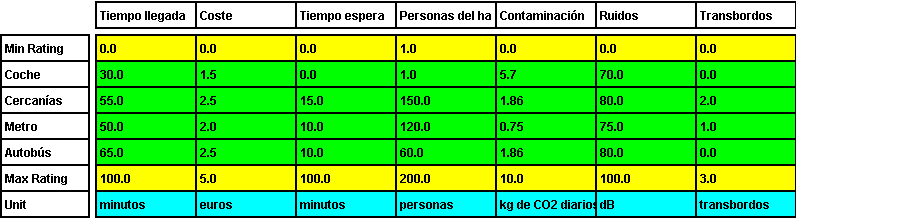
\includegraphics[width=\linewidth]{imagenes/ratings}
	\caption{Ratings de los objetivos terminales}
	\label{fig:ratings}
\end{figure}

En el tiempo de llegada, el coste, el número de transbordos, el tiempo de espera se han considerado los valores máximos y mínimos haciendo una estimación, teniendo una referencia para cada alternativa.\\

En los casos de la contaminación y los ruidos, se han tenido que consultar distintas fuentes para establecer los límites inferior y superior, y dar un valor para cada alternativa.\\

Sólo notar que para el coste, hemos supuesto que nuestro coche consume 5 litros por cada 100 kilómetros, y que el precio del combustible es de 1 euro por litro, dando un resultado de 1.5 euros por trayecto.\\ 

En el caso de la contaminación, los valores para cada alternativa se han calculado con la calculadora de CO2 de Terra \url{http://www.terra.org/calc/}. Notar que esta calculadora necesita la distancia recorrida (en kilómetros) y el número de veces que se realiza el trayecto. En nuestro caso son 30 kilómetros y una vez al día (sólo consideramos el trayecto de ida). Aplicando los parámetros para cada transporte y dividiendo entre 365 (calcula los kilogramos de CO2 emitidos en un año), se obtienen los valores de la Figura~\ref{fig:ratings}.\\

En el caso del ruido, marcamos el límite máximo como 100, por debajo del umbral del dolor situado en 120 dB, según la OMS. Para establecer medidas para cada una de las alternativas, consultamos distintas páginas web y blogs, que nos llevan a los datos de la Figura~\ref{fig:ratings}.\\

Ya estamos en disposición de introducir las funciones de valor para cada uno de los objetivos.\\

Comenzamos con el coste. Usando el método Valuefn, creamos una función de valor de tipo exponencial donde se le da al coche como valor 0.979, al metro 0.961 y, al Cercanías y al autobús, 0.930. Es decir, consideramos diferencias mínimas entre los precios de los medios de transporte (Figura~\ref{fig:prioridades_coste}).\\

\begin{figure}[tbph!]
	\centering
	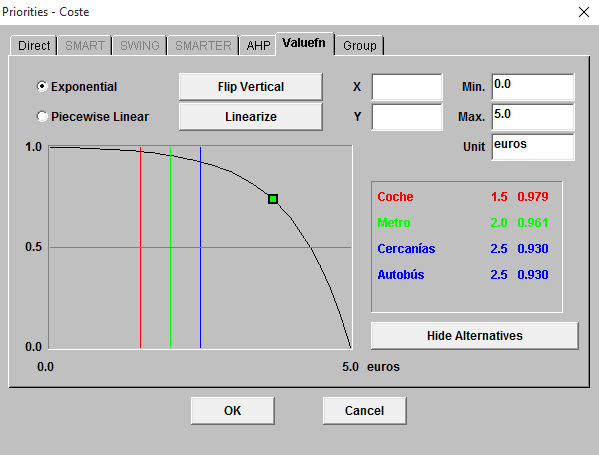
\includegraphics[width=0.5\linewidth]{imagenes/prioridades_coste}
	\caption{Función de valor del coste}
	\label{fig:prioridades_coste}
\end{figure}

En el caso del tiempo de llegada, el número de transbordos, el tiempo de espera, personas del habitáculo, la contaminación y el ruido calculamos la función de valor empleando el mismo método, Valuefn. Las funciones de valor de cada uno de estos objetivos se pueden ver en la Figura~\ref{fig:prioridades}.\\

\begin{figure}[htbp!]
\centering
\subfigure[Función de valor del tiempo de llegada]{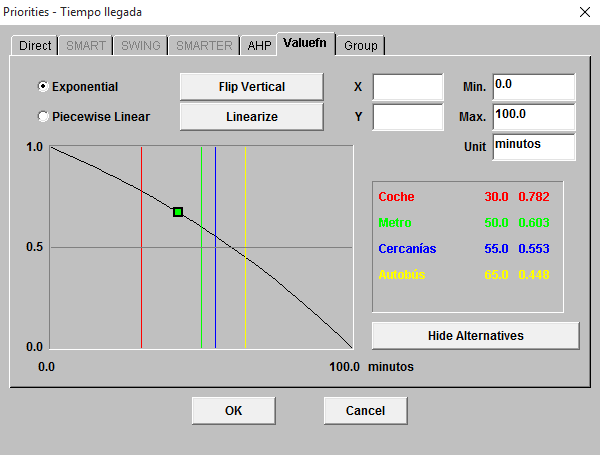
\includegraphics[width=0.4\linewidth]{imagenes/prioridades_tiempo_llegada}}
\subfigure[Función de valor del número de transbordos]{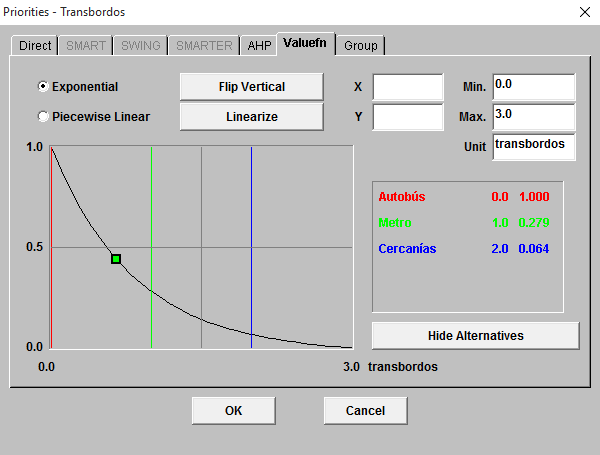
\includegraphics[width=0.4\linewidth]{imagenes/prioridades_transbordos}}
\subfigure[Función de valor del tiempo de espera]{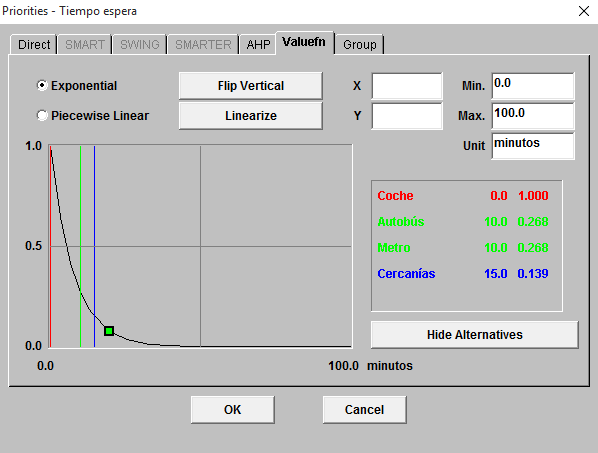
\includegraphics[width=0.4\linewidth]{imagenes/prioridades_tiempo_espera}}
\subfigure[Función de valor del número de personas del habitáculo]{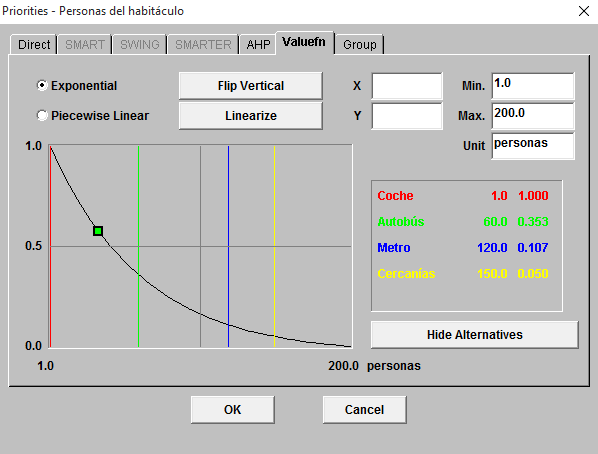
\includegraphics[width=0.4\linewidth]{imagenes/prioridades_personas_del_habitaculo}}
\subfigure[Función de valor de la contaminación]{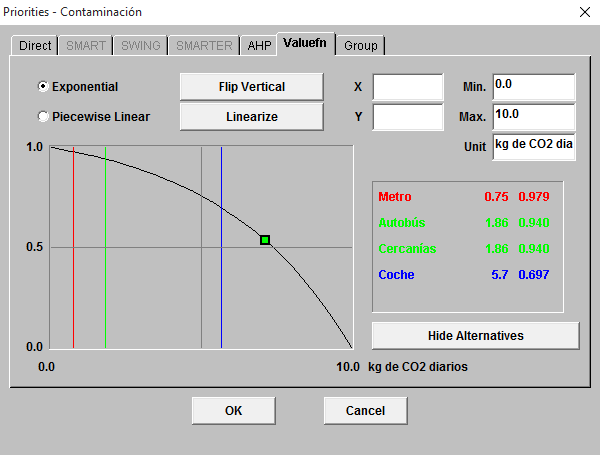
\includegraphics[width=0.4\linewidth]{imagenes/prioridades_contaminacion}}
\subfigure[Función de valor del ruido]{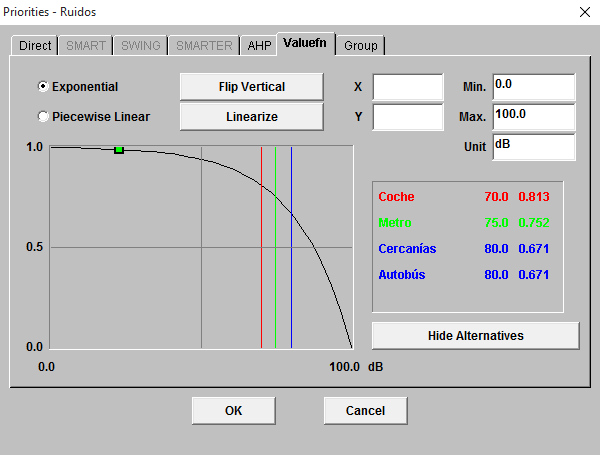
\includegraphics[width=0.4\linewidth]{imagenes/prioridades_ruidos}}
\caption{Funciones de valor para tiempo de llegada, el número de transbordos, el tiempo de espera, personas del habitáculo, la contaminación y el ruido} \label{fig:prioridades}
\end{figure}

Para el caso de los tipos de transporte, terrestre y subterráneo, empleamos el método Direct para asignar la función de valor. Notar que todas las alternativas no son medios de transporte subterráneo y terrestre simultáneamente, sino que sólo pueden ser de un solo tipo. Por ello, sólo unimos el tipo de transporte con sus alternativas correctas (coche y autobús para terrestre, y Cercanías y metro para subterráneo). De esta forma, asignamos pesos a los medios de transporte correctos. La Figura~\ref{fig:prioridades_t_transporte} muestra los pesos para terrestre y subterráneo.\\

\begin{figure}[htbp!]
\centering
\subfigure[Función de valor de terrestre]{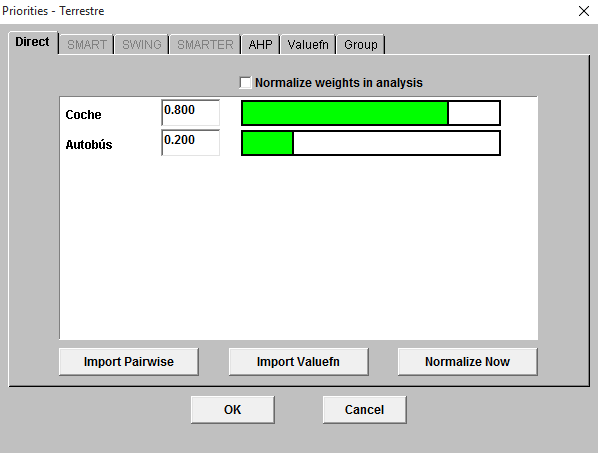
\includegraphics[width=0.4\linewidth]{imagenes/prioridades_terrestre}}
\subfigure[Función de valor de subterráneo]{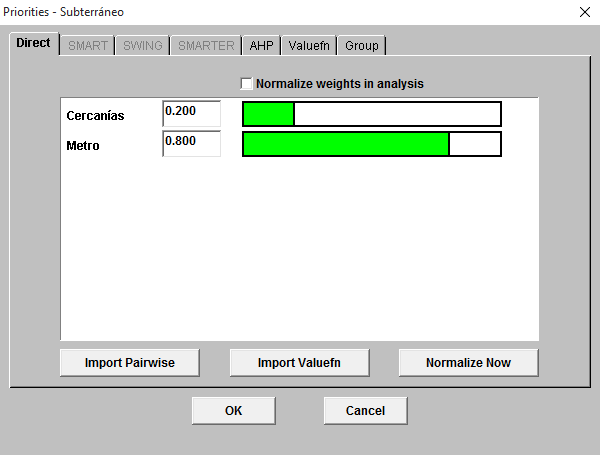
\includegraphics[width=0.4\linewidth]{imagenes/prioridades_subterraneo}}
\caption{Pesos para terrestre y subterráneo} \label{fig:prioridades_t_transporte}
\end{figure}

Para la asignación de prioridades en el caso del tipo de transporte, usamos el modo SWING, donde hay que asignar 100 puntos a la opción más prioritaria (terrestre en nuestro) y dar otra puntuación (menor que 100) a las otras opciones (sólo nos queda la opción de subterráneo a la que damos 40 puntos). Ver Figura~\ref{fig:prioridades_tipo_transporte}.\\

\begin{figure}[htbp!]
\centering
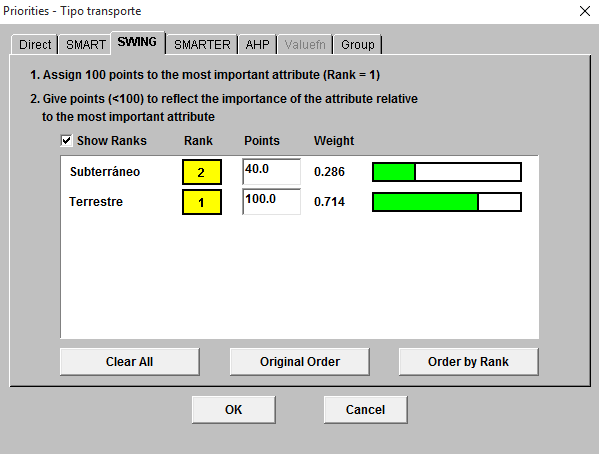
\includegraphics[width=0.5\linewidth]{imagenes/prioridades_tipo_transporte}
\caption{Pesos para tipo de transporte} \label{fig:prioridades_tipo_transporte}
\end{figure}

De nuevo, usamos el método SWING para ajustar los pesos del objetivo Económicos y Confort. En el caso de Económicos asignamos 100 puntos a la opción Tiempo llegada y 40 puntos al coste. Para Confort, asignamos 100 puntos a Tipo transporte, 80 al tiempo de espera, 70 al número de transbordos y 40 al número de personas del habitáculo. Ver Figura~\ref{fig:swing_2}.

\begin{figure}[htbp!]
\centering
\subfigure[Asignación de pesos para Ecónomicos]{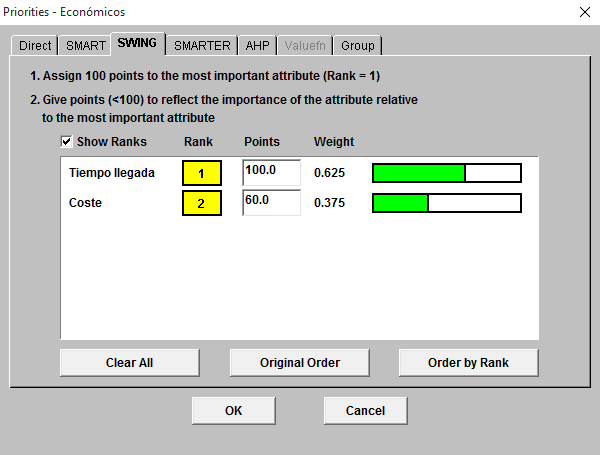
\includegraphics[width=0.4\linewidth]{imagenes/prioridades_economicos}}
\subfigure[Asignación de pesos para Confort]{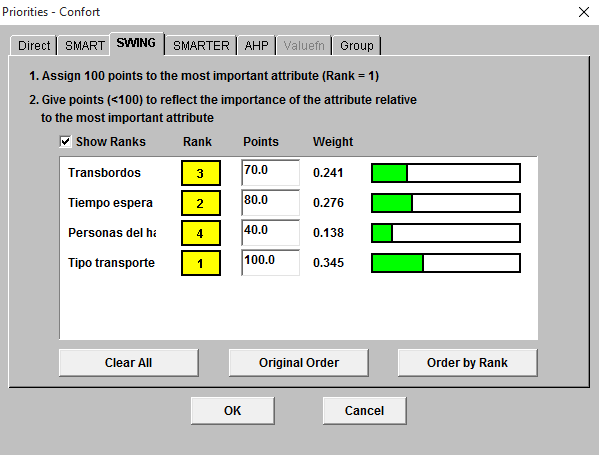
\includegraphics[width=0.4\linewidth]{imagenes/prioridades_confort}}
\caption{Pesos para Económicos y Confort} \label{fig:swing_2}
\end{figure}

Para el objetivo Sociales, asignamos los pesos con el método Direct. Damos 0.8 a la contaminación y 0.2 a los ruidos (Figura~\ref{fig:prioridades_sociales}).\\

\begin{figure}[htbp!]
\centering
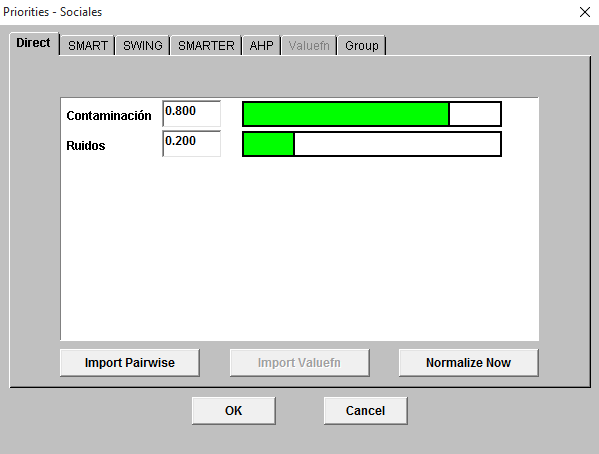
\includegraphics[width=0.5\linewidth]{imagenes/prioridades_sociales}
\caption{Pesos para Sociales} \label{fig:prioridades_sociales}
\end{figure}

Por último, sólo nos queda asignar pesos al objetivo de elegir medio de transporte. Usamos, de nuevo, el método SWING. Damos 100 puntos al objetivos Económicos, 60 a Confort y 45 a Sociales.\\

\begin{figure}[htbp!]
\centering
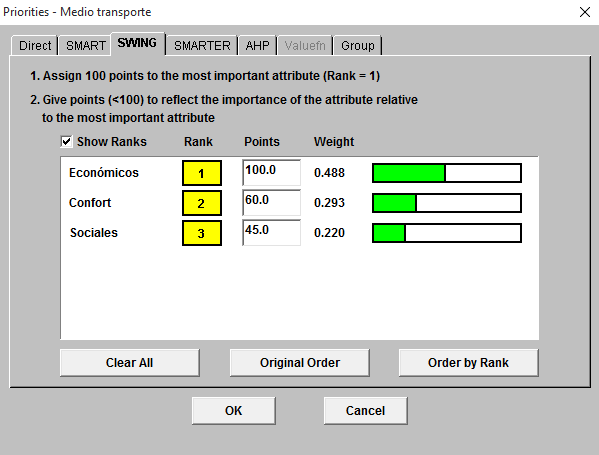
\includegraphics[width=0.5\linewidth]{imagenes/prioridades_medio_transporte}
\caption{Asignación de pesos para Medio de transporte} \label{fig:prioridades_medio_transporte}
\end{figure}

Ya tenemos asignadas las prioridades a todos los objetivos. Ahora debemos analizar nuestras preferencias. La Figura~\ref{fig:analisis_1} muestra los resultados según los objetivos primarios. Observamos que nuestra opción preferida es el coche, seguido del metro y el autobús. En última opción se encuentra Cercanías. De acuerdo a lo establecido anteriormente, los objetivos económicos pesan mucho para la elección de la alternativa.\\

\begin{figure}[htbp!]
\centering
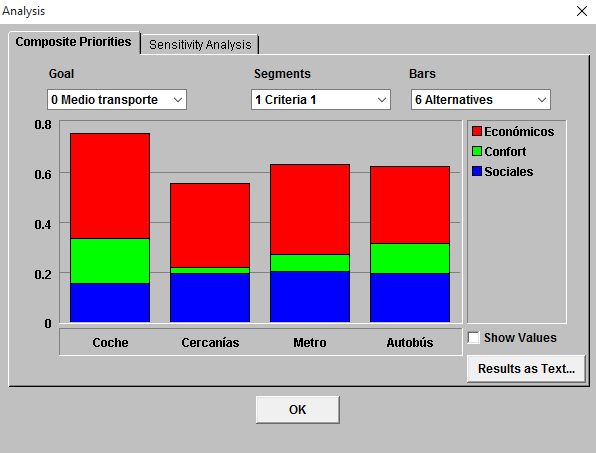
\includegraphics[width=0.5\linewidth]{imagenes/analisis_1}
\caption{Preferencias según objetivos Económicos, Confort y Sociales} \label{fig:analisis_1}
\end{figure}

Si, por último, consideramos los resultados según los objetivos terminales (Figura~\ref{fig:analisis_2}) observamos que lo que más peso tiene dentro de nuestras preferencias es el tiempo de llegada, seguido del coste, y en menor medida, la contaminación.\\

\begin{figure}[htbp!]
\centering
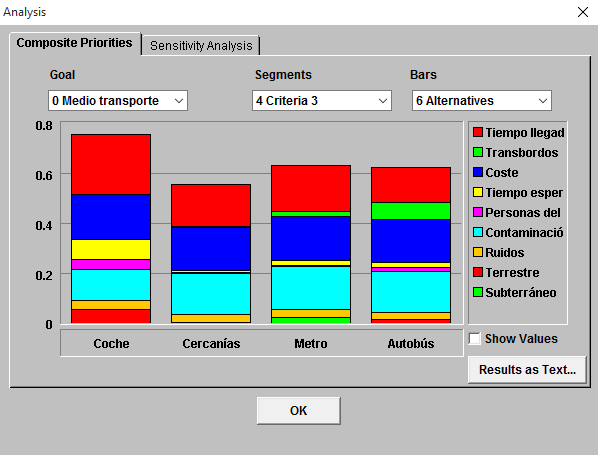
\includegraphics[width=0.5\linewidth]{imagenes/analisis_2}
\caption{Preferencias según objetivos terminales} \label{fig:analisis_2}
\end{figure}

\subsection{Optimización}

Antes de poder optimizar, necesitamos cohesionar nuestros dos modelos: el diagrama de influencia y el modelo jerárquico de objetivos (Figura~\ref{fig:diagrama_influencia_completo}).\\

\begin{figure}[htbp!]
\centering
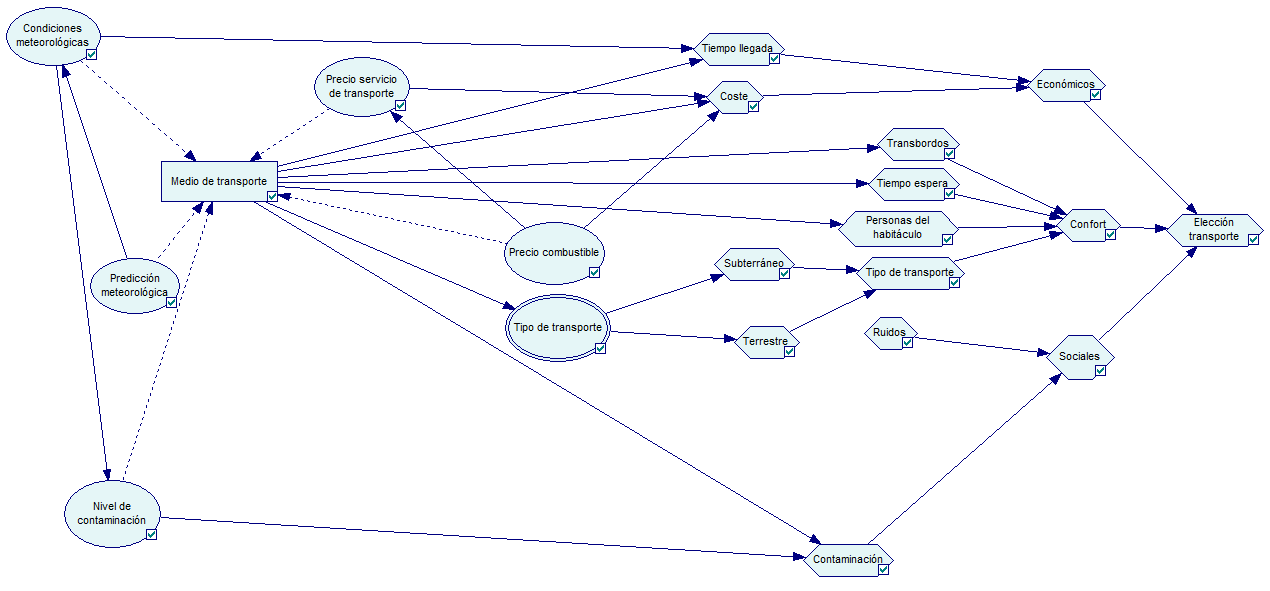
\includegraphics[width=\linewidth]{imagenes/diagrama_influencia_completo}
\caption{Modelo completo} \label{fig:diagrama_influencia_completo}
\end{figure}

Observamos la inclusión de un nodo determinístico llamado Tipo de transporte para distinguir entre los medios de transporte terrestres y subterráneos. En la Figura~\ref{fig:tipo_de_transporte} se muestran los distintos valores de este nodo.\\ 

\begin{figure}[htbp!]
\centering
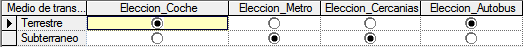
\includegraphics[width=0.6\linewidth]{imagenes/tipo_de_transporte}
\caption{Valores del nodo determinístico Tipo de transporte} \label{fig:tipo_de_transporte}
\end{figure}

Ya podemos introducir los valores en los nodos de valor obtenidos con Web-HIPRE.\\

Resolvemos el modelo con GeNIe, obteniendo los resultados que se muestran en la Figura~\ref{fig:solucion}.

\begin{figure}[htbp!]
\centering
\subfigure[Solución para condiciones meteorológicas de lluvia]{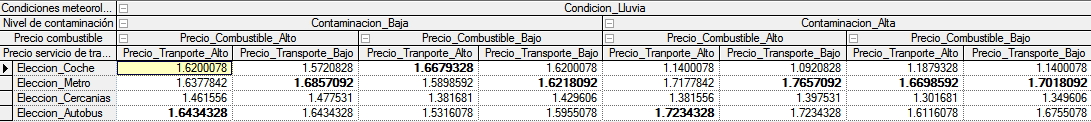
\includegraphics[width=\linewidth]{imagenes/solucion_lluvia}}
\subfigure[Solución para condiciones meteorológicas de nieve]{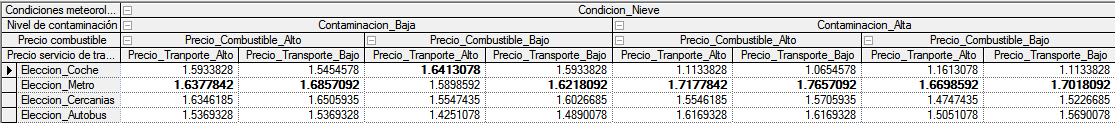
\includegraphics[width=\linewidth]{imagenes/solucion_nieve}}
\subfigure[Solución para condiciones meteorológicas de niebla]{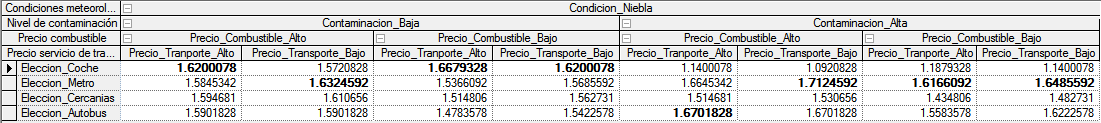
\includegraphics[width=\linewidth]{imagenes/solucion_niebla}}
\subfigure[Solución para condiciones meteorológicas con el cielo despejado]{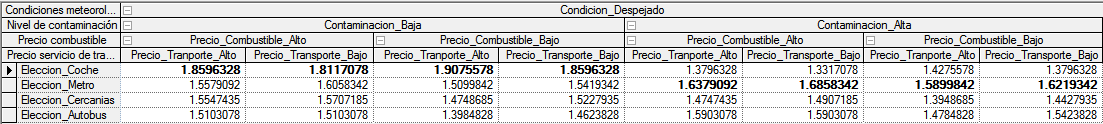
\includegraphics[width=\linewidth]{imagenes/solucion_despejado}}
\caption{Solución del modelo} \label{fig:solucion}
\end{figure}

\subsection{Análisis del modelo}

Puesto que la solución tiene muchas incertidumbres, representamos, en forma de árbol, para cada condición meteorológica el medio de transporte que da la solución. Ver~\Cref{fig:sol_lluvia,fig:sol_nieve,fig:sol_niebla,fig:sol_despejado}. En cada una de las figuras se indica en azul las condiciones meteorológicas, en amarillo el nivel de contaminación, en verde el precio del combustible y, en rojo el precio del transporte.\\

\begin{figure}[htbp!]
\centering
\begin{tikzpicture}[
level 1/.style={sibling distance=60mm},
level 2/.style={sibling distance=30mm},
level 3/.style={sibling distance=15mm},
level 4/.style={sibling distance=8mm},
every text node part/.style={align=center},
scale=1.25
]
\node[c,fill=blue!20] {Lluvia}
    child{ node[c, fill=yellow!20]  {Baja} edge from parent[onearrow]
            child{ node[c, fill=green!20] {Alto} 
                    child{ node[c, fill=red!20] {Alto} 
                        child{ node[r] {Autobús} edge from parent} 
                    }
                    child{ node[c, fill=red!20] {Bajo} edge from parent[onearrow]
                        child{ node[r] {Metro} edge from parent}
                    }
            }
            child{ node [c, fill=green!20] {Bajo} edge from parent[onearrow]
                    child{ node[c, fill=red!20] {Alto}  edge from parent[onearrow]
                        child{ node[r] {Coche} edge from parent} 
                    }
                    child{ node[c, fill=red!20] {Bajo} edge from parent[onearrow]
                        child{ node[r] {Metro} edge from parent} 
                    }
            }
    }
    child{ node[c,fill=yellow!20] {Alta} edge from parent[onearrow]
            child{ node [c, fill=green!20] {Alto} edge from parent
                    child{ node[c, fill=red!20] {Alto} 
                        child{ node[r] {Autobús} edge from parent[onearrow]} 
                    }
                    child{ node[c, fill=red!20] {Bajo} edge from parent[onearrow]
                        child{ node[r] {Metro} edge from parent} 
                    }
            }
            child{ node [c, fill=green!20] {Bajo} edge from parent[onearrow]
                    child{ node[c, fill=red!20] {Alto} edge from parent
                        child{ node[r] {Metro} edge from parent[onearrow]} 
                    }
                    child{ node[c, fill=red!20] {Bajo} edge from parent[onearrow]
                        child{ node[r] {Metro} edge from parent} 
                    }
            }
    }
;
\end{tikzpicture}
\caption{Árbol con la solución para condiciones de lluvia}
\label{fig:sol_lluvia}
\end{figure}

En el caso de condiciones de lluvia (Figura~\ref{fig:sol_lluvia}), debemos utilizar distintos medios de transporte según el nivel de contaminación, el precio del combustible y de los transportes públicos. Así, en caso de contaminación baja, precio del combustible alto y precio del transporte público alto debemos escoger el autobús. Si tenemos el precio del transporte público bajo, entonces el metro. Si hay contaminación baja, precio del combustible alto y el precio del transporte público es alto, entonces cogeremos el coche. Si el precio del transporte es bajo, debemos elegir el metro. Si la contaminación es alta, el precio del combustible alto, el precio del transporte alto, entonces el autobús cogeremos. Si el precio del transporte es bajo cogeremos el metro. Si el precio del combustible es bajo, entonces escogeremos el metro, independientemente del precio del transporte público.\\

\begin{figure}[htbp!]
\centering
\begin{tikzpicture}[
level 1/.style={sibling distance=60mm},
level 2/.style={sibling distance=30mm},
level 3/.style={sibling distance=15mm},
level 4/.style={sibling distance=8mm},
every text node part/.style={align=center},
scale=1.25
]
\node[c,fill=blue!20] {Nieve}
    child{ node[c, fill=yellow!20]  {Baja} edge from parent[onearrow]
            child{ node[c, fill=green!20] {Alto} 
                    child{ node[c, fill=red!20] {Alto} 
                        child{ node[r] {Metro} edge from parent} 
                    }
                    child{ node[c, fill=red!20] {Bajo} edge from parent[onearrow]
                        child{ node[r] {Metro} edge from parent}
                    }
            }
            child{ node [c, fill=green!20] {Bajo} edge from parent[onearrow]
                    child{ node[c, fill=red!20] {Alto}  edge from parent[onearrow]
                        child{ node[r] {Coche} edge from parent} 
                    }
                    child{ node[c, fill=red!20] {Bajo} edge from parent[onearrow]
                        child{ node[r] {Metro} edge from parent} 
                    }
            }
    }
    child{ node[c,fill=yellow!20] {Alta} edge from parent[onearrow]
            child{ node [c, fill=green!20] {Alto} edge from parent
                    child{ node[c, fill=red!20] {Alto} 
                        child{ node[r] {Metro} edge from parent[onearrow]} 
                    }
                    child{ node[c, fill=red!20] {Bajo} edge from parent[onearrow]
                        child{ node[r] {Metro} edge from parent} 
                    }
            }
            child{ node [c, fill=green!20] {Bajo} edge from parent[onearrow]
                    child{ node[c, fill=red!20] {Alto} edge from parent
                        child{ node[r] {Metro} edge from parent[onearrow]} 
                    }
                    child{ node[c, fill=red!20] {Bajo} edge from parent[onearrow]
                        child{ node[r] {Metro} edge from parent} 
                    }
            }
    }
;
\end{tikzpicture}
\caption{Árbol con la solución para condiciones de nieve}
\label{fig:sol_nieve}
\end{figure}

En el caso de condiciones de nieve (Figura~\ref{fig:sol_nieve}), elegiremos siempre el metro, salvo cuando se dé que el nivel de contaminación sea baja, el precio del combustible sea bajo y el precio del transporte público sea alto, que elegiremos el coche.\\

\begin{figure}[htbp!]
\centering
\begin{tikzpicture}[
level 1/.style={sibling distance=60mm},
level 2/.style={sibling distance=30mm},
level 3/.style={sibling distance=15mm},
level 4/.style={sibling distance=8mm},
every text node part/.style={align=center},
scale=1.25
]
\node[c,fill=blue!20] {Niebla}
    child{ node[c, fill=yellow!20]  {Baja} edge from parent[onearrow]
            child{ node[c, fill=green!20] {Alto} 
                    child{ node[c, fill=red!20] {Alto} 
                        child{ node[r] {Coche} edge from parent} 
                    }
                    child{ node[c, fill=red!20] {Bajo} edge from parent[onearrow]
                        child{ node[r] {Metro} edge from parent}
                    }
            }
            child{ node [c, fill=green!20] {Bajo} edge from parent[onearrow]
                    child{ node[c, fill=red!20] {Alto}  edge from parent[onearrow]
                        child{ node[r] {Coche} edge from parent} 
                    }
                    child{ node[c, fill=red!20] {Bajo} edge from parent[onearrow]
                        child{ node[r] {Coche} edge from parent} 
                    }
            }
    }
    child{ node[c,fill=yellow!20] {Alta} edge from parent[onearrow]
            child{ node [c, fill=green!20] {Alto} edge from parent
                    child{ node[c, fill=red!20] {Alto} 
                        child{ node[r] {Autobús} edge from parent[onearrow]} 
                    }
                    child{ node[c, fill=red!20] {Bajo} edge from parent[onearrow]
                        child{ node[r] {Metro} edge from parent} 
                    }
            }
            child{ node [c, fill=green!20] {Bajo} edge from parent[onearrow]
                    child{ node[c, fill=red!20] {Alto} edge from parent
                        child{ node[r] {Metro} edge from parent[onearrow]} 
                    }
                    child{ node[c, fill=red!20] {Bajo} edge from parent[onearrow]
                        child{ node[r] {Metro} edge from parent} 
                    }
            }
    }
;
\end{tikzpicture}
\caption{Árbol con la solución para condiciones de niebla}
\label{fig:sol_niebla}
\end{figure}

En caso de niebla (Figura~\ref{fig:sol_niebla}), si tenemos contaminación baja, escogeremos el coche, salvo cuando el precio del combustible sea alto y el precio del transporte público bajo. En caso de que haya contaminación alta, elegiremos siempre el metro, salvo cuando el precio del combustible sea alto y el precio del transporte público sea alto que escogeremos el autobús.\\

\begin{figure}[htbp!]
\centering
\begin{tikzpicture}[
level 1/.style={sibling distance=60mm},
level 2/.style={sibling distance=30mm},
level 3/.style={sibling distance=15mm},
level 4/.style={sibling distance=8mm},
every text node part/.style={align=center},
scale=1.25
]
\node[c,fill=blue!20] {Desp.}
    child{ node[c, fill=yellow!20]  {Baja} edge from parent[onearrow]
            child{ node[c, fill=green!20] {Alto} 
                    child{ node[c, fill=red!20] {Alto} 
                        child{ node[r] {Coche} edge from parent} 
                    }
                    child{ node[c, fill=red!20] {Bajo} edge from parent[onearrow]
                        child{ node[r] {Coche} edge from parent}
                    }
            }
            child{ node [c, fill=green!20] {Bajo} edge from parent[onearrow]
                    child{ node[c, fill=red!20] {Alto}  edge from parent[onearrow]
                        child{ node[r] {Coche} edge from parent} 
                    }
                    child{ node[c, fill=red!20] {Bajo} edge from parent[onearrow]
                        child{ node[r] {Coche} edge from parent} 
                    }
            }
    }
    child{ node[c,fill=yellow!20] {Alta} edge from parent[onearrow]
            child{ node [c, fill=green!20] {Alto} edge from parent
                    child{ node[c, fill=red!20] {Alto} 
                        child{ node[r] {Metro} edge from parent[onearrow]} 
                    }
                    child{ node[c, fill=red!20] {Bajo} edge from parent[onearrow]
                        child{ node[r] {Metro} edge from parent} 
                    }
            }
            child{ node [c, fill=green!20] {Bajo} edge from parent[onearrow]
                    child{ node[c, fill=red!20] {Alto} edge from parent
                        child{ node[r] {Metro} edge from parent[onearrow]} 
                    }
                    child{ node[c, fill=red!20] {Bajo} edge from parent[onearrow]
                        child{ node[r] {Metro} edge from parent} 
                    }
            }
    }
;
\end{tikzpicture}
\caption{Árbol con la solución para condiciones de cielo despejado}
\label{fig:sol_despejado}
\end{figure}

En caso de que el cielo esté despejado (Figura~\ref{fig:sol_despejado}), escogeremos el coche si hay contaminación baja y el metro si la contaminación es alta.\\

\subsection{Análisis de sensibilidad}

A continuación, realizamos un análisis de sensibilidad con Web-HIPRE. A tenor de nuestras elección de preferencias, los modos de asignación más imprecisos son Direct y SWING. Debemos estudiar como varían nuestras preferencias en los nodos cuyos método de asignación de preferencias sea alguno de los dos anteriores. Por brevedad, solo comentaremos cómo cambia la solución del nodo Medio Transporte si cambian las preferencias de los objetivos Económicos, Confort y Sociales (Figura~\ref{fig:sensibilidad}).\\


\begin{figure}[htbp!]
\centering
\subfigure[Análisis de sensibilidad del objetivo Económicos]{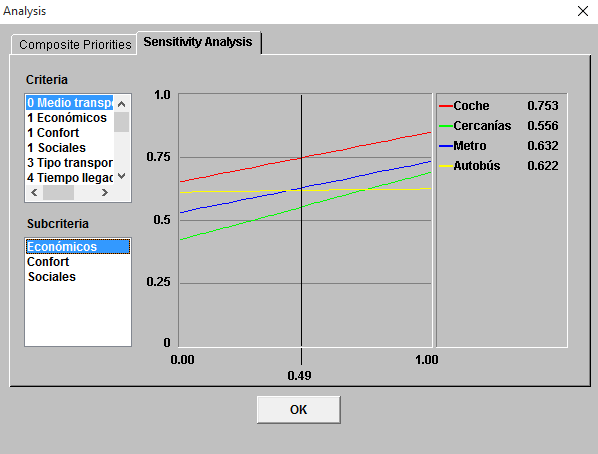
\includegraphics[width=0.4\linewidth]{imagenes/sen_economicos}}
\subfigure[Análisis de sensibilidad del objetivo Económicos]{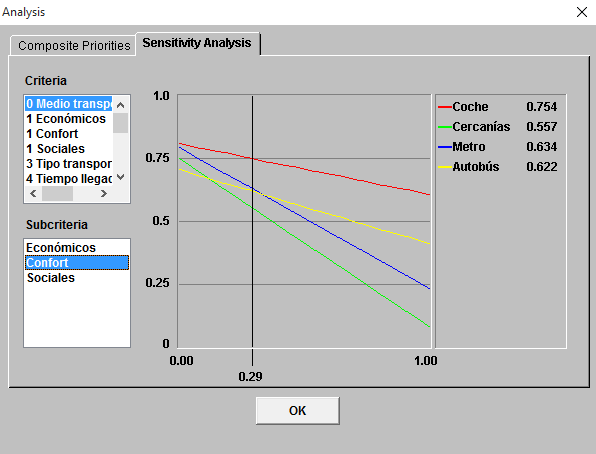
\includegraphics[width=0.4\linewidth]{imagenes/sen_confort}}
\subfigure[Análisis de sensibilidad del objetivo Económicos]{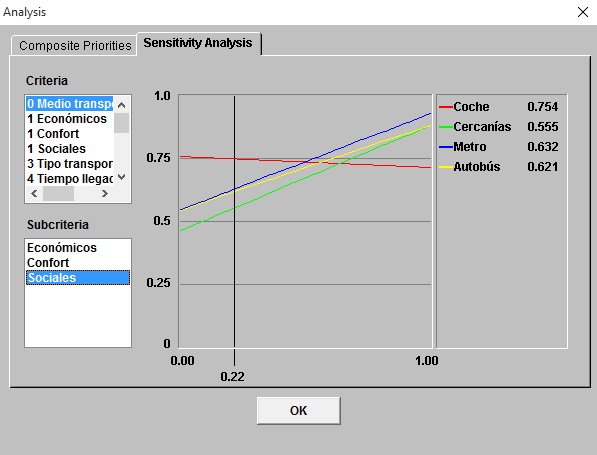
\includegraphics[width=0.4\linewidth]{imagenes/sen_sociales}}
\caption{Análisis de sensibilidad} \label{fig:sensibilidad}
\end{figure}

En el caso del objetivo Económicos, la función de valor cambia bastante. Las preferencias de coche se mueven entre 0.60 y 0.85, del autobús oscilan entre 0.57 y 0.58, en el caso del metro entre 0.53 y 0.75 y de Cercanías entre 0.45 y 0.70.\\

En el caso del objetivo Confort, también se producen muchas variaciones en torno a la función de valor: en el caso del coche los valores varían entre 0.77 y 0.60. En el metro varían de 0.76 a 0.45, en el Cercanías de 0.75 a 0.15 y en el autobús de 0.74 a 0.24.\\

Por último, en el caso de los objetivos Sociales también se producen cambios pero algo menos acusados. En el caso del coche, los valores varían entre 0.75 y 0.70, en el metro de 0.55 a 0.95, en el autobús de 0.55 a 0.90 y el Cercanías de 0.47 a 0.90.\\

En general, se observa mucha variación de las preferencias en estos tres objetivos, aunque la más acusada se ve en el objetivo de Confort. Puede ser debido a la subjetividad con la que hemos definido cómo se mide el confort (número de transbordos, tipo de transporte, tiempo de llegada, etc).\\

Ahora introducimos estos nuevos valores para ver cómo cambia la solución del problema en GeNIe.\\

Al resolver el modelo con estos nuevos valores, la solución no varía, salvo en el caso de condiciones de lluvia: si tenemos contaminación baja, combustible alto y precio del transporte alto ahora deberemos elegir coche en vez del autobús.

\section{Conclusiones}

Hemos resuelto el problema de la ruta óptima para llegar al trabajo siguiendo el ciclo del análisis de decisiones. Para tomar nuestra decisión debemos de tener en cuenta las condiciones meteorológicas y los precios del combustible y de los transportes públicos. Debido a nuestras preferencias, los medios de transporte que más utilizaremos para llegar al trabajo serán el coche y el metro, y en algún caso excepcional, el autobús.\\

Esta solución puede variar mucho debido a la naturaleza del problema: es muy subjetivo definir qué es el confort y cómo medirlo (hemos usado parámetros como número de transbordos, número de personas del habitáculo, tipo de transporte y tiempo de espera). Otro decisor, con otras preferencias opuestas a las nuestras, podría obtener una solución totalmente distinta de la nuestra.\\

El modelo se podría mejorar distinguiendo distintos niveles para las condiciones meteorológicas. Por ejemplo, en el caso de la lluvia, podríamos tener chubascos dispersos, lluvia suave e intensa, etc. De esta manera seríamos nuestro modelo más robusto y preciso.\\

Por último, cabe destacar la utilización de dos software: GeNIe y Web-HIPRE. El primero de ellos, permite crear, modificar y resolver diagramas de influencia de una forma sencilla y rápida, ahorrando mucho tiempo durante el modelado. El segundo, permite evaluar nuestras preferencias creando un modelo jerárquico de objetivos. También tiene una interfaz muy sencilla que permite obtener las preferencias de forma muy gráfica, obteniendo una fácil interpretación.  

\end{document} 